\begin{exercise}
\begin{figure}[H]
\centering

\includegraphics[width=\textwidth]{hw14-2025060321.png}
% \caption{}
\label{}
\end{figure}
\begin{figure}[H]
\centering
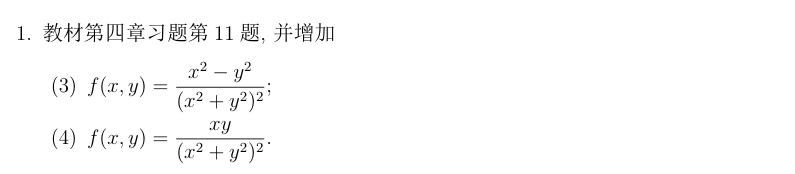
\includegraphics[width=\textwidth]{1-hw14-2025060321.png}
% \caption{}
\label{}
\end{figure}
\end{exercise}
\begin{figure}[H]
\centering
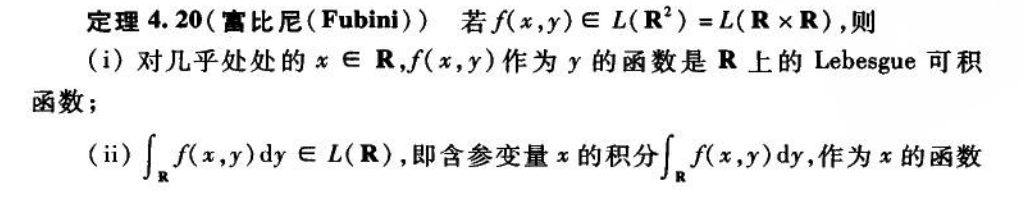
\includegraphics[width=\textwidth]{14-hw14-2025060321.png}
% \caption{}
\label{}
\end{figure}
\begin{figure}[H]
\centering
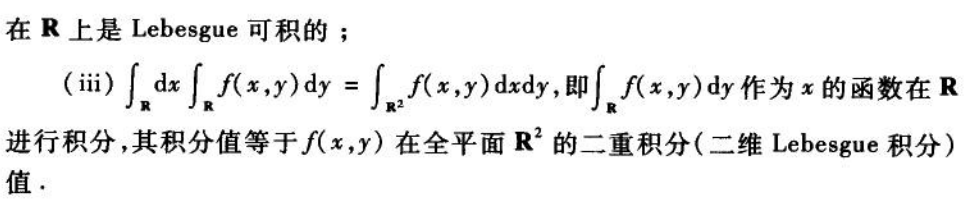
\includegraphics[width=\textwidth]{15-hw14-2025060321.png}
% \caption{}
\label{}
\end{figure}
事实上我们只要验证
\[
\int_{[-1,1]^2}^{} \lvert f(x,y) \rvert  \, \mathrm{d}x\mathrm{d}y<\infty
\]
即可,也就是
\[
\int_{[-1,1]^2}^{} \left\lvert  \frac{x^2-y^2}{x^2+y^2}  \right\rvert  \, \mathrm{d}x \mathrm{d}y<\infty
\]
事实上
\[
\int_{[-1,1]^2}^{} \left\lvert  \frac{x^2-y^2}{x^2+y^2}  \right\rvert  \, \mathrm{d}x \mathrm{d}y=2 (-2 + \pi)<\infty
\]
满足 Fubini 定理的条件. 两个累次积分分别为
\[
\int_{[-1,1]}^{} \int_{[-1,1]}^{} \frac{x^2-y^2}{x^2+y^2} \, \mathrm{d}x  \, \mathrm{d}y =\int_{[-1,1]}^{} 2-4y\arctan\left( \frac{1}{y} \right) \, \mathrm{d}y=0 
\]
\[
\int_{[-1,1]}^{} \int_{[-1,1]}^{} \frac{x^2-y^2}{x^2+y^2} \, \mathrm{d}y  \, \mathrm{d}x =\int_{[-1,1]}^{} -2+4x\arctan\left( \frac{1}{x} \right) \, \mathrm{d}x =0
\]
相等.

(2)
\[
\int_{[-1,1]^2}^{} \lvert f(x,y) \rvert  \, \mathrm{d}x \mathrm{d}y=\int_{[-1,1]^2}^{}\left\lvert   \frac{xy}{x^2+y^2}  \right\rvert  \, \mathrm{d}x \mathrm{d}y=2\log2<\infty
\]
满足 Fubini 定理的条件.
\[
\int_{[-1,1]}^{} \int_{[-1,1]}^{} \frac{xy}{x^2+y^2} \, \mathrm{d}x  \, \mathrm{d}y =\int_{[-1,1]}^{} 0 \, \mathrm{d}y =0
\]
\[
\int_{[-1,1]}^{} \int_{[-1,1]}^{} \frac{xy}{x^2+y^2} \, \mathrm{d}y  \, \mathrm{d}x =\int_{[-1,1]}^{} 0 \, \mathrm{d}x =0
\]
两个累次积分分别为
\[
\int_{[-1,1]}^{} \int_{[-1,1]}^{} \frac{x^2-y^2}{x^2+y^2} \, \mathrm{d}x  \, \mathrm{d}y =\int_{[-1,1]}^{} 2-4y\arctan\left( \frac{1}{y} \right) \, \mathrm{d}y=0 
\]
\[
\int_{[-1,1]}^{} \int_{[-1,1]}^{} \frac{x^2-y^2}{x^2+y^2} \, \mathrm{d}y  \, \mathrm{d}x =\int_{[-1,1]}^{} -2+4x\arctan\left( \frac{1}{x} \right) \, \mathrm{d}x =0
\]
相等.

(3)
\[
\begin{aligned}
\int_{[-1,1]^2}^{} \lvert f(x,y) \rvert  \, \mathrm{d}x \mathrm{d}y & =\int_{[-1,1]^2}^{} \left\lvert  \frac{x^2-y^2}{(x^2+y^2)^2}  \right\rvert  \, \mathrm{d}x \mathrm{d}y \\
 & \geq \int_{\epsilon}^{1} \int_{0}^{2\pi}   r \cdot \left\lvert  \frac{r^2\cos ^2\theta-r^2\sin ^2\theta}{r^{4}}  \right\rvert  \, \mathrm{d}\theta  \, \mathrm{d}r  \\
 & =\int_{\epsilon}^{1} \frac{1}{r} \, \mathrm{d}r \cdot\underbrace{  \int_{0}^{2\pi} \lvert \cos2\theta \rvert  \, \mathrm{d}\theta    }_{ =4  } \\
 & =4\ln\frac{1}{\epsilon} \\
 & \to \infty \qquad \text{as }\epsilon\to0^{+} 
\end{aligned} 
\]
不满足Fubini 定理的条件. 两个累次积分分别为
\[
\int_{[-1,1]}^{} \int_{[-1,1]}^{} \frac{x^2-y^2}{(x^2+y^2)^2} \, \mathrm{d}x  \, \mathrm{d}y =\int_{[-1,1]}^{} -\frac{2}{1+y^2} \, \mathrm{d}y= -\pi
\]
\[
\int_{[-1,1]}^{} \int_{[-1,1]}^{} \frac{x^2-y^2}{(x^2+y^2)^2} \, \mathrm{d}y  \, \mathrm{d}x=\int_{[-1,1]}^{} \frac{2}{1+x^2} \, \mathrm{d}x =\pi
\]
不相等.

(4)
\[
\begin{aligned}
\int_{[-1,1]^2}^{} \lvert f(x,y) \rvert  \, \mathrm{d}x \mathrm{d}y & =\int_{[-1,1]^2}^{} \left\lvert  \frac{xy}{(x^2+y^2)^2}  \right\rvert  \, \mathrm{d}x \mathrm{d}y \\
 & \geq \int_{\epsilon}^{1} \int_{0}^{2\pi} r\left\lvert  \frac{r^2\sin\theta \cos\theta}{r^{4}}  \right\rvert  \, \mathrm{d}\theta  \, \mathrm{d}r  \\
 & =\int_{\epsilon}^{1} \frac{1}{r} \, \mathrm{d}r \cdot \int_{0}^{2\pi} \lvert \sin\theta \cos\theta \rvert  \, \mathrm{d}\theta     \\
 & =2\ln\frac{1}{\epsilon} \\
 & \to \infty \qquad \text{as }\epsilon\to0^{+} 
\end{aligned}
\]
不满足 Fubini 定理的条件. 两个累次积分分别为
\[
\int_{[-1,1]}^{} \int_{[-1,1]}^{}  \frac{xy}{(x^2+y^2)^2}  \, \mathrm{d}x  \, \mathrm{d}y= \int_{[-1,1]}^{} 0 \, \mathrm{d}y=0
\]
\[
\int_{[-1,1]}^{} \int_{[-1,1]}^{}  \frac{xy}{(x^2+y^2)^2}  \, \mathrm{d}y  \, \mathrm{d}x= \int_{[-1,1]}^{} 0 \, \mathrm{d}x=0
\]
相等.

\begin{exercise}
\begin{figure}[H]
\centering

\includegraphics[width=\textwidth]{2-hw14-2025060321.png}
% \caption{}
\label{}
\end{figure}
\end{exercise}
只需验证
\[
\int_F I_\lambda(x) \mathrm{d} x<\infty
\]
注意到当 $y \in F$ 时,$\delta(y)=0$ .故有
\[
I_\lambda(x)=\int_{\mathbb{R}} \frac{\delta(y)^\lambda}{|x-y|^{1+\lambda}} \mathrm{d} y=\int_{F^c} \frac{\delta(y)^\lambda}{|x-y|^{1+\lambda}} \mathrm{d} y
\]
因为被积函数 $\frac{\delta(y)^\lambda}{|x-y|^{1+\lambda}}$ 在 $\left\{(x, y) \in \mathbb{R}^2: x \neq y\right\}$ 内连续,所以在 $\mathbb{R}^2$ 上可测.由 Tonelli 定理可得
\[
\int_F I_\lambda(x) \mathrm{d} x=\int_F\left(\int_{F^c} \frac{\delta(y)^\lambda}{|x-y|^{1+\lambda}} \mathrm{d} y\right) \mathrm{d} x=\int_{F^c} \delta(y)^\lambda\left(\int_F \frac{\mathrm{~d} x}{|x-y|^{1+\lambda}}\right) \mathrm{d} y
\]
由于 $F$ 中的任意点到 $y$ 的距离都 $\geqslant \delta(y)$ ,故有 $F \subset(-\infty, y-\delta(y)] \cup[y+\delta(y),+\infty)$ .
于是
\[
\begin{aligned}
\int_F \frac{\mathrm{~d} x}{|x-y|^{1+\lambda}} & \leqslant \int_{(-\infty, y-\delta(y)] \cup[y+\delta(y),+\infty)} \frac{\mathrm{d} x}{|x-y|^{1+\lambda}} \\
& =\int_{-\infty}^{y-\delta(y)} \frac{\mathrm{d} x}{|x-y|^{1+\lambda}}+\int_{y+\delta(y)}^{\infty} \frac{\mathrm{d} x}{|x-y|^{1+\lambda}}
\end{aligned}
\]
上式右端的 Lebesgue 积分可归结为广义 Riemann 积分计算得
\[
\begin{aligned}
& (R) \int_{-\infty}^{y-\delta(y)} \frac{\mathrm{d} x}{|x-y|^{1+\lambda}}+(R) \int_{y+\delta(y)}^{\infty} \frac{\mathrm{d} x}{|x-y|^{1+\lambda}} \\
= & (R) \int_{-\infty}^{-\delta(y)} \frac{\mathrm{d} t}{|t|^{1+\lambda}}+(R) \int_{\delta(y)}^{\infty} \frac{\mathrm{d} t}{|t|^{1+\lambda}}=2 \cdot(R) \int_{\delta(y)}^{\infty} \frac{\mathrm{d} t}{t^{1+\lambda}}=\frac{2}{\lambda \delta(y)^\lambda}
\end{aligned}
\]
这样就得到
\[
\int_F \frac{\mathrm{~d} x}{|x-y|^{1+\lambda}} \leqslant \frac{2}{\lambda \delta(y)^\lambda}
\]
进而有
\[
\int_F I_\lambda(x) \mathrm{d} x=\int_{F^c} \delta(y)^\lambda\left(\int_F \frac{\mathrm{~d} x}{|x-y|^{1+\lambda}}\right) \mathrm{d} y \leqslant \int_{F^c} \delta(y)^\lambda \cdot \frac{2}{\lambda \delta(y)^\lambda} \mathrm{d} y=\frac{2}{\lambda} m\left(F^c\right)<\infty
\]
\begin{exercise}
\begin{figure}[H]
\centering
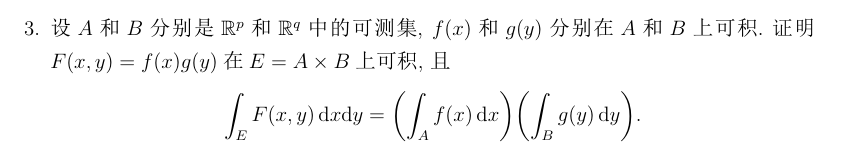
\includegraphics[width=\textwidth]{3-hw14-2025060321.png}
% \caption{}
\label{}
\end{figure}
\end{exercise}
\begin{figure}[H]
\centering
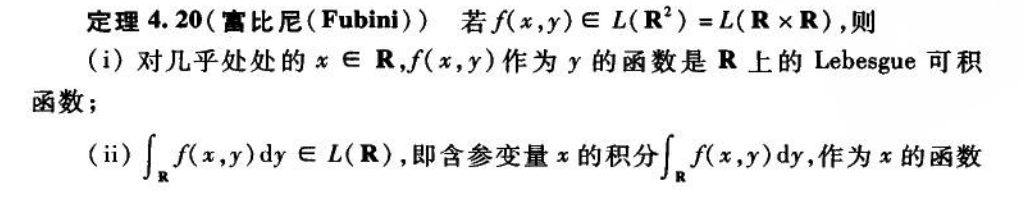
\includegraphics[width=\textwidth]{14-hw14-2025060321.png}
% \caption{}
\label{}
\end{figure}
\begin{figure}[H]
\centering
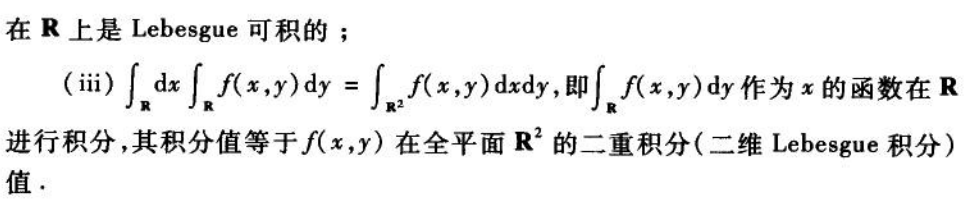
\includegraphics[width=\textwidth]{15-hw14-2025060321.png}
% \caption{}
\label{}
\end{figure}

我们有
\[
\int_{A\times B}^{} \lvert F(x,y) \rvert   \, \mathrm{d}x \mathrm{d}y=\int_{A\times B}^{} \lvert f(x) \rvert \cdot \lvert g(y) \rvert  \, \mathrm{d}x \mathrm{d}y\overset{ \text{Tonelli} }{ = }\int_{A}^{} \lvert f(x) \rvert  \, \mathrm{d}x \cdot \int_{B}^{} \lvert g(y) \rvert  \, \mathrm{d}y<\infty
\]
于是可以应用 Fubini 定理,得到
\[
\int_{E}^{} F(x,y) \, \mathrm{d}x \mathrm{d}y=\left( \int_{A}^{} f(x) \, \mathrm{d}x  \right)\left( \int_{B}^{} g(y) \, \mathrm{d}y  \right)
\]
\begin{exercise}
\begin{figure}[H]
\centering
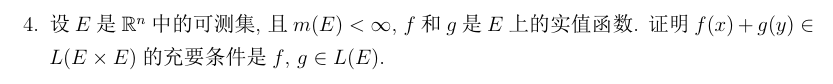
\includegraphics[width=\textwidth]{4-hw14-2025060321.png}
% \caption{}
\label{}
\end{figure}
\end{exercise}
若 $f, g\in L(E)$,则
\[
\begin{aligned}
\int_{E\times E}^{} \lvert f(x)+g(y) \rvert  \, \mathrm{d}x \mathrm{d}y & \leq \int_{E\times E}^{} \lvert f(x) \rvert +\lvert g(y) \rvert  \, \mathrm{d}x \mathrm{d}y \\
 & =\int_{E\times E}^{ } \lvert f(x) \rvert  \, \mathrm{d}x \mathrm{d}y+\int_{E\times E}^{} \lvert g(y) \rvert  \, \mathrm{d}x \mathrm{d}y \\
 & \overset{ \text{Tonelli} }{ = }m(E)\cdot(\lVert f \rVert _{L^{1}(E)}+\lVert g \rVert _{L^{1}(E)})  \\
 & <\infty
\end{aligned}
\]
故 $f (x)+g (y)\in L(E\times E)$.

若 $f (x)+g (y)\in L(E\times E)$,
\[
\int_{E\times E}^{} \lvert f(x)+g(y) \rvert  \, \mathrm{d}x \mathrm{d}y<\infty
\]
由 Fubini 定理可知
\[
\int_{E}^{}\underbrace{  \int_{E}^{} \lvert f(x)+g(y) \rvert  \, \mathrm{d}y  }_{ \eqqcolon \varphi(x) } \, \mathrm{d}x <\infty
\]
由于 $\varphi (x)\in L(E)$,故 $\varphi(x)$ 在 $E$ 上几乎处处有限,给定 $x_0$ 使得 $\varphi(x_0)$ 有限,因为 $f (x_0)+g (y)\in L(E)$,故 $f(x_0)+g(y)$ 在 $E$ 上几乎处处有限,故 $g(y)$ 在 $E$ 上几乎处处有限. 同理, $f(x)$ 在 $E$ 上几乎处处有限. 选取 $x_0\in E$ 使得 $\varphi(x_0)$ 和 $f(x_0)$ 都有限,那么
\[
\int_{E}^{} \lvert g(y) \rvert  \, \mathrm{d}y \leq \int_{E}^{} \lvert f(x_0)+g(y) \rvert  \, \mathrm{d}y +\int_{E}^{} \lvert f(x_0) \rvert  \, \mathrm{d}x =\varphi(x_0)+\lvert f(x_0) \rvert \cdot m(E)<\infty
\]
故 $g\in L(E)$,同理 $f\in L(E)$.

\begin{exercise}
\begin{figure}[H]
\centering
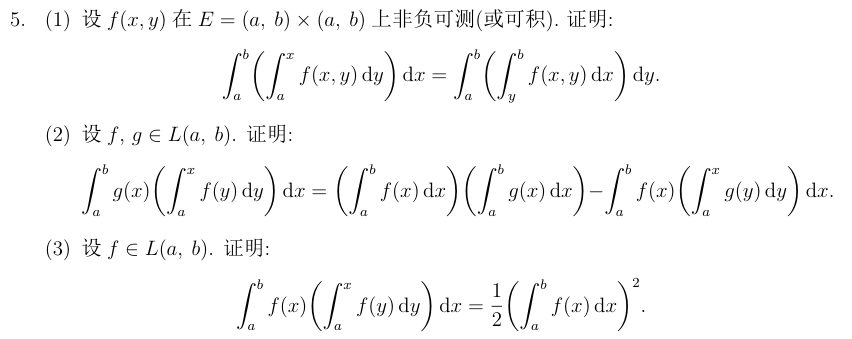
\includegraphics[width=\textwidth]{5-hw14-2025060321.png}
% \caption{}
\label{}
\end{figure}
\end{exercise}
(1)
\[
\begin{aligned}
\int_{a}^{b} \left( \int_{a}^{x} f(x,y) \, \mathrm{d}y  \right) \, \mathrm{d}x  & =\int_{a}^{b} \left( \int_{a}^{b} f(x,y) \chi_{x\geq y}\, \mathrm{d}y  \right) \, \mathrm{d}x  \\
 & \overset{ \text{Tonelli}  }{ = }\int_{a}^{b} \left( \int_{a}^{b} f(x,y)\chi_{x\geq y} \, \mathrm{d}x  \right) \, \mathrm{d}y \\
  & =\int_{a}^{b} \left( \int_{y}^{b} f(x,y) \, \mathrm{d}x  \right) \, \mathrm{d}y  
\end{aligned}
\]
(2)
要证明:$f (x) g (y)\in L(E\times E)$. 这是因为
\[
\int_{[a,b]^2}^{} \lvert f(x)g(y) \rvert  \, \mathrm{d}x \mathrm{d}y\overset{ \text{Tonelli} }{ = }\int_{[a,b]}^{} \lvert f(x) \rvert  \, \mathrm{d}x \cdot \int_{[a,b]}^{} \lvert g(y) \rvert  \, \mathrm{d}y <\infty
\]
所以
\[
\begin{aligned}
\left( \int_{a}^{b} f(x)\, \mathrm{d}x \right) \left( \int_{a}^{b} g(x) \, \mathrm{d}x \right)  & =\int_{a}^{b} f(x)\left( \int_{a}^{b} g(y) \, \mathrm{d}y  \right)\, \mathrm{d}x \\
 & =\int_{a}^{b} f(x)\left( \int_{a}^{x} g(y) \, \mathrm{d}y+\int_{x}^{b} g(y) \, \mathrm{d}y   \right) \, \mathrm{d} x \\
  & =\int_{a}^{b} f(x)\left( \int_{a}^{x} g(y) \, \mathrm{d}y  \right) \, \mathrm{d}x +\int_{a}^{b} f(x) \left( \int_{x}^{b} g(y) \, \mathrm{d}y  \right) \, \mathrm{d}x  \\
 & =\int_{a}^{b} f(x)\left( \int_{a}^{x} g(y) \, \mathrm{d}y  \right) \, \mathrm{d}x +\int_{[a,b]^2}^{} f(x)g(y)\chi_{x\geq y} \, \mathrm{d}x \mathrm{d}y \\
 & =\int_{a}^{b} f(x)\left( \int_{a}^{x} g(y) \, \mathrm{d}y  \right) \, \mathrm{d}x +\int_{a}^{b} g(x) \left( \int_{a}^{x} f(y) \, \mathrm{d}y  \right)\, \mathrm{d}x 
\end{aligned}
\]
(3)
在 (2) 中令 $g=f$ 即可.

\begin{exercise}
\begin{figure}[H]
\centering

\includegraphics[width=\textwidth]{6-hw14-2025060321.png}
% \caption{}
\label{}
\end{figure}
\begin{figure}[H]
\centering
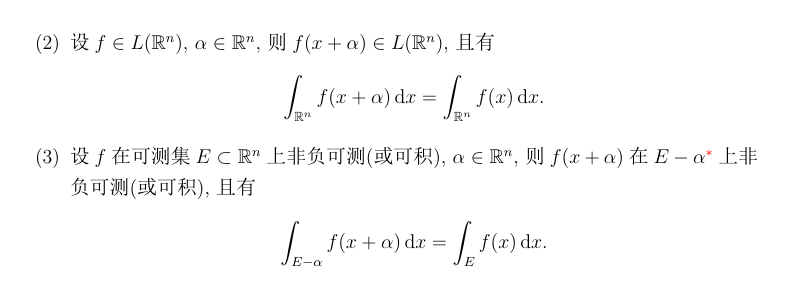
\includegraphics[width=\textwidth]{7-hw14-2025060321.png}
% \caption{}
\label{}
\end{figure}
\end{exercise}
(1)
\[
\begin{aligned}
\int_{(-R+\alpha _1,R-\alpha_1)\times\dots \times(-R+\alpha _n,R-\alpha _n)}^{} f(x+\alpha) \, \mathrm{d}x  & \overset{ \text{Tonelli} }{ = }\prod_{i=1}^{n} \int_{(-R+\alpha _i,R-\alpha _i)}^{} f(x_i) \, \mathrm{d}x_i   \\
 & \leq \prod_{i=1}^{n} \int_{(-R,R)}^{} f(x_i) \, \mathrm{d}x_i \\ 
 & \overset{ \text{Tonelli} }{ = } \int_{(-R,R)^{n}}^{}f(x)  \, \mathrm{d}x   \\
 & \leq \prod_{i=1}^{n} \int_{(-R-\alpha _i,R+\alpha _i)}^{} f(x_i) \, \mathrm{d}x_i \\
 & \overset{ \text{Tonelli} }{ = } \int_{(-R-\alpha _1,R+\alpha_1)\times\dots \times(-R-\alpha _n,R+\alpha _n)}^{} f(x+\alpha) \, \mathrm{d}x
\end{aligned}
\]
令 $R\to \infty$,就有 $\int_{\mathbb{R}^{n}}^{} f(x+\alpha) \, \mathrm{d}x=\int_{\mathbb{R}^{n}}^{} f(x) \, \mathrm{d}x$.

(2)
同理,利用 Fubini 定理即可.

(3)
同上,拆分成各个分量上的积分,再用变量代换即可.

\begin{exercise}
\begin{figure}[H]
\centering

\includegraphics[width=\textwidth]{10-hw14-2025060321.png}
% \caption{}
\label{}
\end{figure}
\begin{figure}[H]
\centering
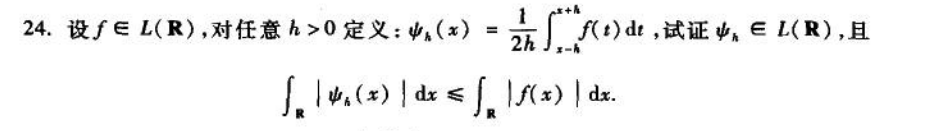
\includegraphics[width=\textwidth]{8-hw14-2025060321.png}
% \caption{}
\label{}
\end{figure}
\end{exercise}
\[
\begin{aligned}
\int_{\mathbb{R}}^{} \lvert \psi_{h}(x) \rvert  \, \mathrm{d}x  & =\int_{\mathbb{R}}^{} \left\lvert  \frac{1}{2h}\int_{x-h}^{x+h} f(t) \, \mathrm{d}t   \right\rvert  \, \mathrm{d}x  \\
 & \leq \frac{1}{2h}\int_{\mathbb{R}}^{} \int_{[-h,h]}^{} \lvert f(x+t) \rvert  \, \mathrm{d}t  \, \mathrm{d}x  \\
 & \overset{ \text{Tonelli} }{ = }\frac{1}{2h}\int_{[-h,h]}^{} \int_{\mathbb{R}}^{} \lvert f(x+t) \rvert  \, \mathrm{d}x  \, \mathrm{d}t \\
  & =\frac{1}{2h}\int_{[-h,h]}^{} \int_{\mathbb{R}}^{} \lvert f(x) \rvert  \, \mathrm{d}x  \, \mathrm{d}t \\
  & =\int_{\mathbb{R}}^{} \lvert f(x) \rvert  \, \mathrm{d}x  \\
 & <\infty
\end{aligned}
\]
于是 $\psi_{h}\in L(\mathbb{R})$.

\begin{exercise}
\begin{figure}[H]
\centering
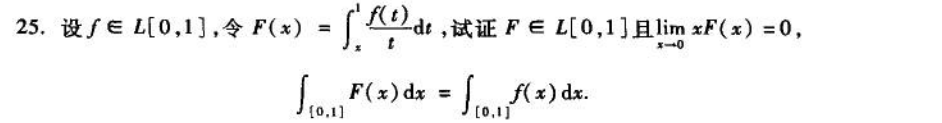
\includegraphics[width=\textwidth]{9-hw14-2025060321.png}
% \caption{}
\label{}
\end{figure}
\end{exercise}
首先
\[
\begin{aligned}
\int_{[0,1]}^{} \lvert F(x) \rvert  \, \mathrm{d}x  & \leq \int_{[0,1]}^{} \int_{[x,1]}^{} \left\lvert  \frac{f(t)}{t}  \right\rvert  \, \mathrm{d}t  \, \mathrm{d}x  \\
 & =\int_{[0,1]^2}^{} \left\lvert  \frac{f(t)}{t}  \right\rvert  \chi_{t\geq x}\, \mathrm{d}x \mathrm{d}t \\
 & =\int_{[0,1]}^{} \int_{[0,t]}^{} \left\lvert  \frac{f(t)}{t}  \right\rvert  \, \mathrm{d}x  \, \mathrm{d}t  \\
 & =\int_{[0,1]}^{ } \lvert f(t) \rvert  \, \mathrm{d}t \\
  & <\infty
\end{aligned}
\]
于是 $F\in L[0,1]$.

利用积分的绝对连续性
\[
\begin{aligned}
\lvert xF(x) \rvert  & =\left\lvert  x\int_{x}^{1} \frac{f(t)}{t} \, \mathrm{d}t  \right\rvert  \\
 & \leq \int_{x}^{1} \left\lvert  \frac{x}{t}f(t)   \right\rvert \, \mathrm{d}t   \\
 & =\int_{[x,\sqrt{ x }]}^{} \left\lvert  \frac{x}{t}f(t)  \right\rvert  \, \mathrm{d}t+\int_{[\sqrt{ x },1]}^{} \left\lvert  \frac{x}{t}f(t)  \right\rvert  \, \mathrm{d}t  \\
 & \leq \int_{[x,\sqrt{ x }]}^{} \lvert f(t) \rvert  \, \mathrm{d}t +\int_{[\sqrt{ x },1]}^{} \left\lvert  \frac{x}{\sqrt{ x }} f(t) \right\rvert  \, \mathrm{d}t \\
 & \leq  \int_{[x,\sqrt{ x }]}^{} \lvert f(t) \rvert  \, \mathrm{d}t +\sqrt{ x }\cdot\int_{[0,1]}^{} \lvert f(t) \rvert  \, \mathrm{d}t  \\
 & \to0\qquad \text{as }x\to0
\end{aligned}
\]
由于 $\frac{f (t)}{t}\chi_{t\geq x}\in L([0,1]^2)$,所以
\[
\begin{aligned}
\int_{[0,1]}^{} F(x) \, \mathrm{d}x  & =\int_{[0,1]}^{} \int_{[x,1]}^{} \frac{f(t)}{t} \, \mathrm{d}t  \, \mathrm{d}x  \\
 & =\int_{[0,1]^2}^{} \frac{f(t)}{t}\chi_{t\geq x} \, \mathrm{d}t\mathrm{d}x \\
  & =\int_{[0,1]}^{} \int_{0}^{t} \frac{f(t)}{t} \, \mathrm{d}x  \, \mathrm{d}t  \\
 & =\int_{[0,1]}^{} f(t) \, \mathrm{d}t 
\end{aligned} 
\]
\begin{exercise}
\begin{figure}[H]
\centering

\includegraphics[width=\textwidth]{11-hw14-2025060321.png}
% \caption{}
\label{}
\end{figure}
\begin{figure}[H]
\centering
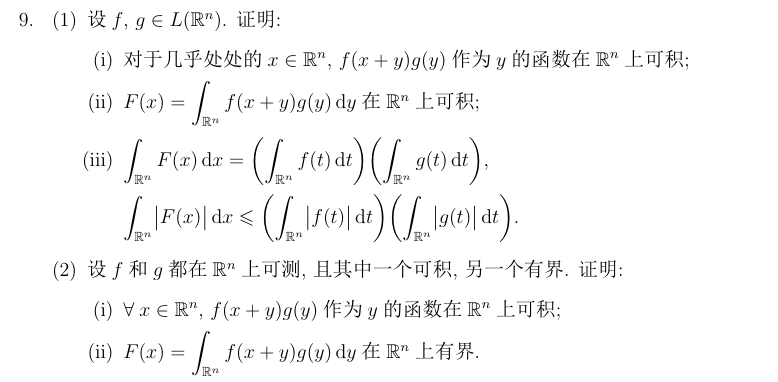
\includegraphics[width=\textwidth]{12-hw14-2025060321.png}
% \caption{}
\label{}
\end{figure}
\end{exercise}
(1)

(i) 显然 $f (x+y) g (y)$ 是 $\mathbb{R}^{n}\times \mathbb{R}^{n}$ 上的可测函数,于是
\[
\int_{\mathbb{R}^{n}\times \mathbb{R}^{n}}^{} \lvert f(x+y)g(y) \rvert  \, \mathrm{d}x \mathrm{d}y=\int_{\mathbb{R}^{n}}^{} \int_{\mathbb{R}^{n}}^{} \lvert f(x+y) \rvert \cdot \lvert g(y) \rvert  \, \mathrm{d}x  \, \mathrm{d}y=\int_{\mathbb{R}^{n}}^{} \lVert f \rVert _{L^{1}(\mathbb{R}^{n})}\cdot \lvert g(y) \rvert  \, \mathrm{d}y=\lVert f \rVert _{L^{1}(\mathbb{R}^{n})}\cdot \lVert g \rVert _{L^{1}(\mathbb{R}^{n})}<\infty  
\]
于是 $f (x+y) g (y)\in L(\mathbb{R}^{n}\times \mathbb{R}^{n})$,与此同时
\[
\int_{\mathbb{R}^{n}\times \mathbb{R}^{n}}^{} \lvert f(x+y)g(y) \rvert  \, \mathrm{d}x \mathrm{d}y\overset{ \text{Tonelli} }{ = }\int_{\mathbb{R}^{n}}^{} \int_{\mathbb{R}^{n}}^{} \lvert f(x+y)g(y) \rvert  \, \mathrm{d}y  \, \mathrm{d}x \eqqcolon \int_{\mathbb{R}^{n}}^{} \varphi(x) \, \mathrm{d}x 
\]
故 $\varphi\in L^{1}(\mathbb{R}^{n})$,于是 $\varphi(x)$ 对于 $x\in \mathbb{R}^{n}$ 几乎处处有限,从而
\[
\varphi(x)=\int_{\mathbb{R}^{n}}^{} \lvert f(x+y)g(y) \rvert  \, \mathrm{d}y<\infty \qquad \text{a.e.}
\]
于是对于几乎处处的 $x\in \mathbb{R}^{n}$,$f(x+y)g(y)$ 作为 $y$ 的函数在 $\mathbb{R}^{n}$ 上可积.

(ii)
已经证明了.

(iii)
\[
\begin{aligned}
\int_{\mathbb{R}^{n}}^{}F(x)  \, \mathrm{d}x & =\int_{\mathbb{R}^{n}}^{} \int_{\mathbb{R}^{n}}^{} f(x+y)g(y) \, \mathrm{d}y \, \mathrm{d}x \\
 &  \overset{ \text{Fubini} }{ = }\int_{\mathbb{R}^{n}}^{} \int_{\mathbb{R}^{n}}^{} f(x+y)g(y) \, \mathrm{d}x  \, \mathrm{d}y \\
 & =\int_{\mathbb{R}^{n}}^{} \lVert f \rVert _{L^{1}(\mathbb{R}^{n})}\cdot g(y)  \, \mathrm{d}y \\
 & =\lVert f \rVert _{L^{1}(\mathbb{R}^{n})}\cdot \lVert g \rVert _{L^{1}(\mathbb{R}^{n})}
\end{aligned}  
\]
\[
\int_{\mathbb{R}^{n}}^{} \lvert F(x) \rvert  \, \mathrm{d}x \leq \int_{\mathbb{R}^{n}}^{} \int_{\mathbb{R}^{n}}^{} \lvert f(x+y)g(y) \rvert  \, \mathrm{d}y  \, \mathrm{d}x \leq \lVert f \rVert _{L^{1}(\mathbb{R}^{n})}\cdot \lVert g \rVert _{L^{1}(\mathbb{R}^{n})}
\]
(2)
由对称性,我们不妨设 $f$ 在 $\mathbb{R}^{n}$ 上有界,$g$ 在 $\mathbb{R}^{n}$ 上可积. 从而对于任意的 $x\in \mathbb{R}^{n}$,我们有
\[
\int_{\mathbb{R}^{n}}^{} \lvert f(x+y)g(y) \rvert  \, \mathrm{d}y \leq M\int_{\mathbb{R}^{n}}^{} \lvert g(y) \rvert  \, \mathrm{d}y<\infty
\]
故 $f(x+y)g(y)$ 作为 $y$ 的函数在 $\mathbb{R}^{n}$ 上可积. 且
\[
\lvert F(x) \rvert \leq \int_{\mathbb{R}^{n}}^{} \lvert f(x+y)g(y) \rvert  \, \mathrm{d}y\leq M\cdot \lVert g \rVert _{L^{1}(\mathbb{R}^{n})}
\]
在 $x\in \mathbb{R}^{n}$ 上有界.

\begin{exercise}
\begin{figure}[H]
\centering
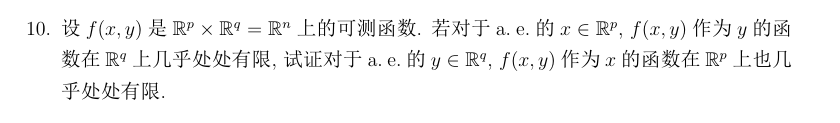
\includegraphics[width=\textwidth]{13-hw14-2025060321.png}
% \caption{}
\label{}
\end{figure}
\end{exercise}
这道题需要用到 Fubini-Tonelli 定理的一个推论,或者直接使用该定理的思想。

\textbf{证明思路:}
我们将考虑函数 $f(x,y)$ 无界的点集,并利用 Fubini-Tonelli 定理来分析这个点集的测度。

\begin{enumerate}
	\item \textbf{定义无界点集}
设 $E = \{ (x,y) \in \mathbb{R}^p \times \mathbb{R}^q : |f(x,y)| = \infty \}$。
由于 $f(x,y)$ 是 $\mathbb{R}^p \times \mathbb{R}^q$ 上的可测函数,那么 $|f(x,y)|$ 也是可测函数。因此,集合 $E$(即 $|f(x,y)|^{-1}(\{\infty\})$)是 $\mathbb{R}^p \times \mathbb{R}^q$ 中的可测集。
	\item \textbf{利用已知条件}
题目给出:对于几乎处处(a.e.)的 $x \in \mathbb{R}^p$,$f(x,y)$ 作为 $y$ 的函数在 $\mathbb{R}^q$ 上几乎处处有限。
这意味着,存在一个零测集 $N_p \subset \mathbb{R}^p$ (即 $m_p(N_p) = 0$),使得对于任意 $x \in \mathbb{R}^p \setminus N_p$,集合
$E_x = \{ y \in \mathbb{R}^q : (x,y) \in E \} = \{ y \in \mathbb{R}^q : |f(x,y)| = \infty \}$
在 $\mathbb{R}^q$ 中是零测集,即 $m_q(E_x) = 0$。
	\item \textbf{应用 Fubini-Tonelli 定理}
考虑集合 $E$ 的指示函数 $\chi_E(x,y)$。由于 $E$ 是可测集,$\chi_E(x,y)$ 是 $\mathbb{R}^p \times \mathbb{R}^q$ 上的非负可测函数。
根据 Tonelli 定理,我们可以计算 $E$ 的测度 $m_{p+q}(E)$:
\[
m_{p+q}(E) = \int_{\mathbb{R}^p \times \mathbb{R}^q} \chi_E(x,y) \,d(x,y) = \int_{\mathbb{R}^p} \left( \int_{\mathbb{R}^q} \chi_E(x,y) \,dy \right) \,dx
\]内层积分 $\int_{\mathbb{R}^q} \chi_E(x,y) \,dy$ 正是 $x$ -截集 $E_x$ 的测度 $m_q(E_x)$。
所以,
\[
m_{p+q}(E) = \int_{\mathbb{R}^p} m_q(E_x) \,dx
\]我们将积分拆开:
\[
m_{p+q}(E) = \int_{\mathbb{R}^p \setminus N_p} m_q(E_x) \,dx + \int_{N_p} m_q(E_x) \,dx
\]根据已知条件,对于 $x \in \mathbb{R}^p \setminus N_p$,我们有 $m_q(E_x) = 0$。因此,第一个积分为 $\int_{\mathbb{R}^p \setminus N_p} 0 \,dx = 0$。
对于第二个积分,由于 $m_p(N_p) = 0$,且 $m_q(E_x) \ge 0$,我们有 $\int_{N_p} m_q(E_x) \,dx = 0$。
(这里我们假设 $m_q(E_x)$ 作为 $x$ 的函数是可测的,这是由 $f$ 的联合可测性保证的,因为 $m_q(E_x)$ 是一个可测函数 $\chi_E$ 的积分切片。)
因此,我们得到 $m_{p+q}(E) = 0 + 0 = 0$。
这意味着集合 $E$ 在 $\mathbb{R}^p \times \mathbb{R}^q$ 中的测度为零。
	\item \textbf{再次应用 Fubini-Tonelli 定理(切换积分次序)}
我们同样有:
\[
m_{p+q}(E) = \int_{\mathbb{R}^q} \left( \int_{\mathbb{R}^p} \chi_E(x,y) \,dx \right) \,dy
\]内层积分 $\int_{\mathbb{R}^p} \chi_E(x,y) \,dx$ 是 $y$ -截集 $E^y = \{ x \in \mathbb{R}^p : (x,y) \in E \}$ 的测度 $m_p(E^y)$。
所以,
\[
m_{p+q}(E) = \int_{\mathbb{R}^q} m_p(E^y) \,dy
\]由于我们已经证明 $m_{p+q}(E) = 0$,所以
\[
\int_{\mathbb{R}^q} m_p(E^y) \,dy = 0
\]因为 $m_p(E^y) \ge 0$ 对所有 $y \in \mathbb{R}^q$ 成立,如果这个非负函数的积分为零,那么它必须几乎处处为零。
即,存在一个零测集 $N_q \subset \mathbb{R}^q$ (即 $m_q(N_q) = 0$),使得对于任意 $y \in \mathbb{R}^q \setminus N_q$,我们有 $m_p(E^y) = 0$。
	\item \textbf{得出结论}
$m_p(E^y) = 0$ 意味着对于 $y \in \mathbb{R}^q \setminus N_q$,集合 $E^y = \{ x \in \mathbb{R}^p : |f(x,y)| = \infty \}$ 在 $\mathbb{R}^p$ 中是零测集。
这正是要证明的结论:对于几乎处处 (a.e.) 的 $y \in \mathbb{R}^q$,$f(x,y)$ 作为 $x$ 的函数在 $\mathbb{R}^p$ 上几乎处处有限。
\end{enumerate}

证毕。
